\subsection{Arquitectura del repositorio de conocimiento}

La arquitectura del repositorio de conocimiento fue diseñada de manera independiente del ecosistema utilizado. Se tomó esta decisión para proveer una interfaz común, independiente de su implementación en IPFS y Ethereum. De esta manera, una aplicación puede trabajar sobre una API común e intercambiar implementaciones fácilmente. Esto es útil para la implementación del front-end del repositorio, como se verá más adelante.

En sí, la arquitectura consiste de una o varias \textit{wikis}, dependiendo de la implementación. Cada wiki se identifica con un nombre único que representa un grupo de artículos en conjunto. Cada wiki se representa con una lista de artículos, los cuales son identificados por sus nombres —también únicos. 

Un artículo se compone de un nombre único y no vacío y su contenido. Si bien nuestra implementación utiliza \textit{markdown} \cite{markdown} como formato del contenido, el tipo de contenido es arbitrario e indiferente para la wiki, cualquier tipo de archivo es admisible. Únicamente será tenido en cuenta en el momento en el que la aplicación que interactúe con el contenido lo interprete. En nuestro caso, markdown representa una manera sencilla de enriquecer un texto, lo cual lo hace apropiado para un repositorio de conocimiento comunitario.

\begin{figure}[H]
    \centering
    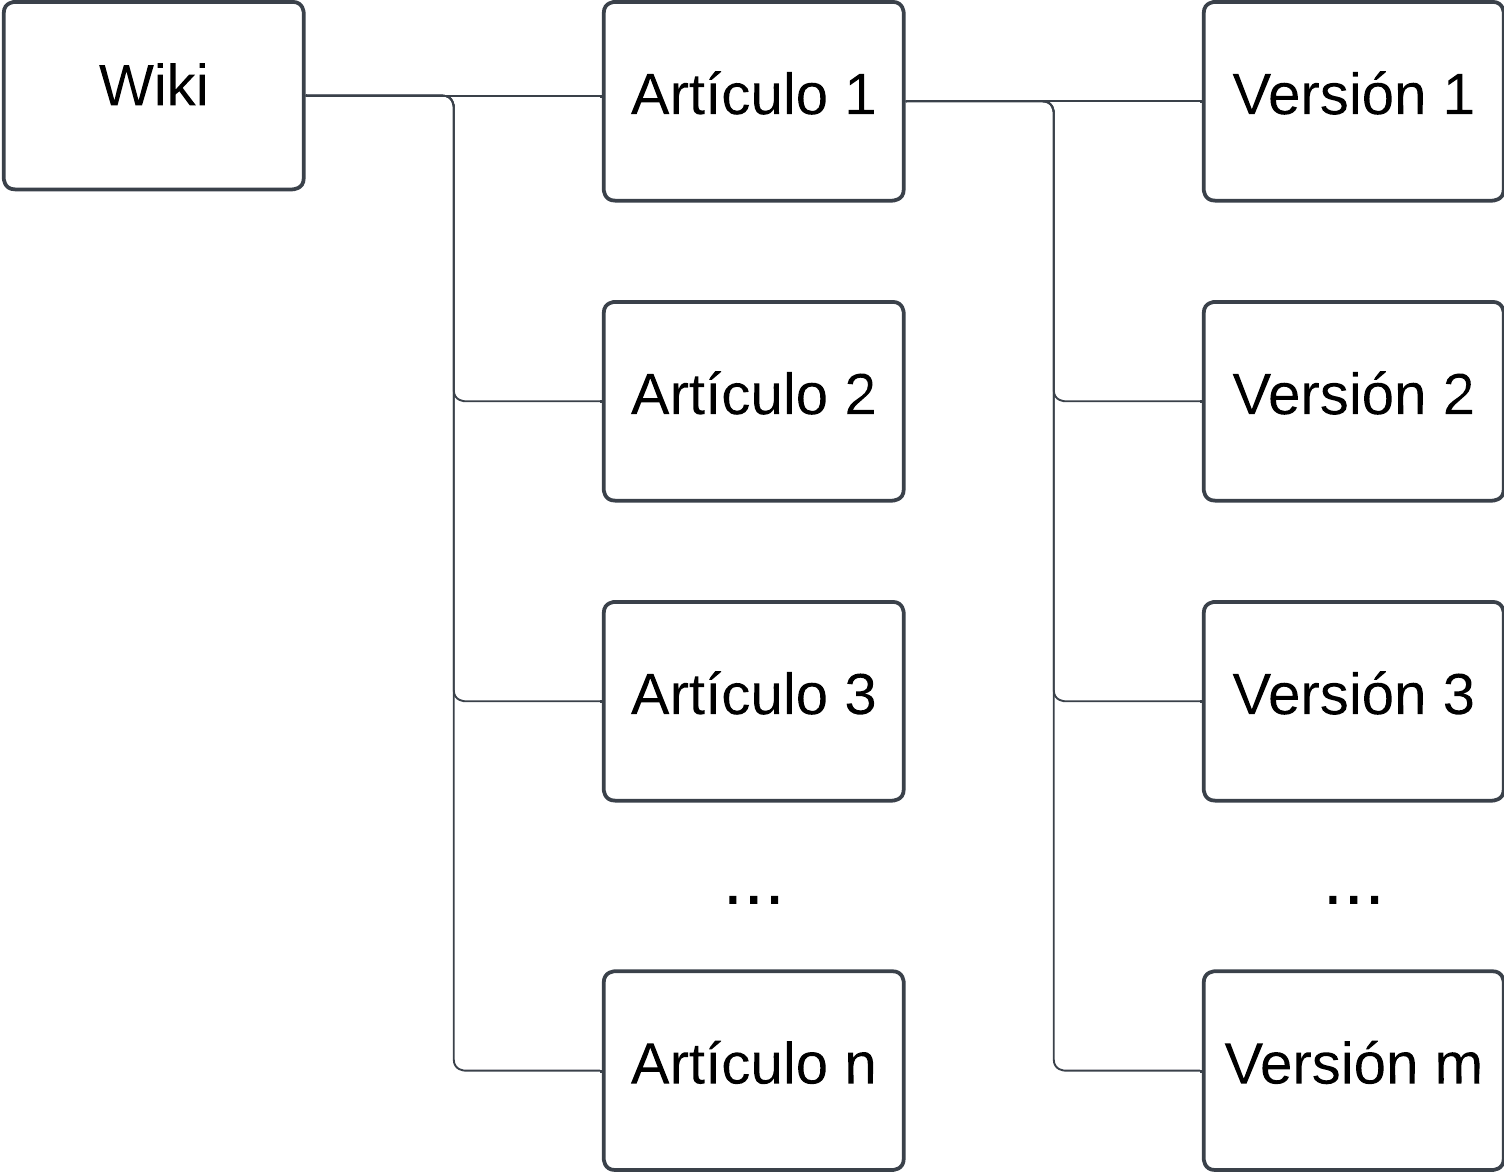
\includegraphics[width=0.5\linewidth]{img/solucion-wiki/arquitectura-wiki.png}
    \caption{Arquitectura general del repositorio de conocimiento.}
    \label{fig:architecture-wiki}
\end{figure}

\subsubsection{Representación de un artículo}

Internamente, los artículos pueden editarse en el tiempo, y un usuario debe obtener siempre la última versión. Sin embargo, se debe poder ver versiones anteriores si así lo desea el usuario, por lo que guardar la última versión únicamente no es válido. Es por esto que se decidió representar a un artículo como un nombre, y un conjunto de versiones. Cada versión representa una modificación hecha al artículo. Un artículo nuevo tendrá una única versión, y al hacerle una edición tendrá dos.

Esta iteración de la arquitectura permite a los usuarios ver el historial de versiones, y acceder a cualquiera de ellas. Pero guardar todo un artículo por cada edición puede ser costoso en concepto de almacenamiento. Rara vez un artículo es modificado en su totalidad \cite{wiki-edits-stats}. En cambio, las ediciones que puede sufrir un artículo se deben en su mayoría a la inclusión de contenido nuevo, o la modificación de una sección en particular. Guardar el contenido completo en casos donde los cambios son mínimos resulta ineficiente, y es particularmente negativo en aplicaciones peer-to-peer, donde el contenido se almacena en el lado del usuario.

\paragraph{Generación de patches}

Como solución para minimizar la información redundante en cada versión, se decidió usar el tipo de algoritmo de \textit{data differencing} \cite{data-differencing}, que consiste en almacenar únicamente los cambios hechos en una versión con respecto a su antecesora, de forma similar a \textit{Git}. Esta lista de cambios forma un \textit{patch}.

Un patch se obtiene al aplicar un algoritmo que reciba el contenido anterior, y el contenido nuevo, y devuelva un patch que pueda ser utilizado posteriormente para reconstruir el contenido. Si bien hay varios algoritmos que logran este objetivo, se decidió utilizar el algoritmo de diff de Myers \cite{myers-diff}, ya que ofrece un punto medio entre compresión, y cómputo necesario para compilar el texto. Este algoritmo es el que utiliza la biblioteca diff-match-patch, creada por Google, que ofrece una interfaz sencilla para lograr generar patches y luego compilar texto en base a ellos.

Calculando los patches de la nueva versión con respecto a la anterior, reducimos el espacio necesario para almacenar un artículo con todas sus versiones.  Hay casos en los que un patch puede tener un tamaño mayor al de simplemente almacenar una copia del nuevo contenido. Sin embargo, estos casos no son frecuentes en usos comunes y decidimos despreciarlos, aunque puede ser una posible mejora para optimizar más aún el espacio utilizado.

Por otra parte, ya que cada versión no tiene toda la información, se necesitan todas las versiones anteriores para compilar el contenido resultante. Esto puede ser una desventaja en archivos con muchas ediciones, ya que requieren de mayor cómputo para compilar, específicamente \texttt{O(n)}, donde \texttt{n} es la cantidad de versiones que tiene el artículo. Para mejorar esto, una posible mejora consiste en fijar un número máximo de patches consecutivos que, al superarse, indica que la siguiente versión debe contener el contenido completo. De esta manera se acota la cantidad de iteraciones que puede tomar la compilación de un artículo.

La nueva iteración de la arquitectura apunta a tener una lista de versiones, que a su vez contengan el patch con las diferencias con la versión anterior. Pero como se verá en la siguiente sección, esta solución no es lo suficientemente resiliente.

\subsubsection{Concurrencia}

En las redes peer-to-peer es común que la replicación de contenido lleve un tiempo no despreciable. Esto puede generar problemas, ya que dos nodos pueden publicar contenido que entre en conflicto, de la misma manera que dos cambios pueden generar un \textit{merge conflict} en Git. En el mejor de los casos, ambos nodos publican
contenido que no entra en conflicto entre sí, y por lo tanto la compilación se puede realizar sin problemas. En el caso contrario, puede dejar el artículo en un estado inválido, imposible de compilar y por lo tanto, inaccesible.

Yendo a nuestro caso de uso, el problema planteado previamente puede entrar en conflicto de dos maneras:
\begin{enumerate}
    \item Al crear un articulo
    \item Al editar un artículo
\end{enumerate}

Por lo tanto, es necesario una solución que mitigue estos problemas.

Para el caso de la creación de dos artículos con en mismo nombre, se delega en cada ecosistema la responsabilidad de detectar estos casos y actuar en consecuencia. La implementación de cada ecosistema contiene más información para tomar una decisión optimizada al respecto, la cuál se verá en secciones posteriores. En cambio, el problema de la edición de un artículo de forma concurrente puede ser resuelto a nivel arquitectura.

\subsubsection{Árbol de versiones}

Hasta ahora, cada versión se agrega a una lista de versiones, y se asume que cada versión se basa en la anterior. Cuando ocurre un conflicto de concurrencia entre versiones, esto no aplica por las razones dadas previamente. Por lo tanto, es necesario que cada versión tenga un ID para que las versiones posteriores puedan mantener registro de su versión padre, es decir, la versión sobre la que se basa. Todas las versiones tienen padre, excepto la versión inicial. Cuando dos versiones se crean en base a una misma versión padre, se genera una bifurcación. Por lo tanto, las versiones pasan a formar un árbol.

En arquitecturas tradicionales, la generación de IDs suele hacerse por la misma base de datos, de manera incremental. Esto no genera problemas ya que el servidor decide en que orden tomar las versiones. En una aplicación distribuida, esto no es conveniente, ya que dos nodos pueden generar el mismo ID por la misma razón por la que pueden generar versiones conflictivas. La solución elegida fue usar \texttt{UUID}s \cite{uuid}, que se generan sin necesidad de centralizar la decisión, y tienen una probabilidad de colisión casi nula.

Una problemática que trae tener distintas ramas de versiones es que la compilación del contenido deja de ser trivial, ya que hay múltiples posibles últimas versiones, dependiendo de la rama que se elija. Para resolver esto es necesario definir una heurística que elija la rama principal del artículo de forma determinista.

\begin{figure}[H]
    \centering
    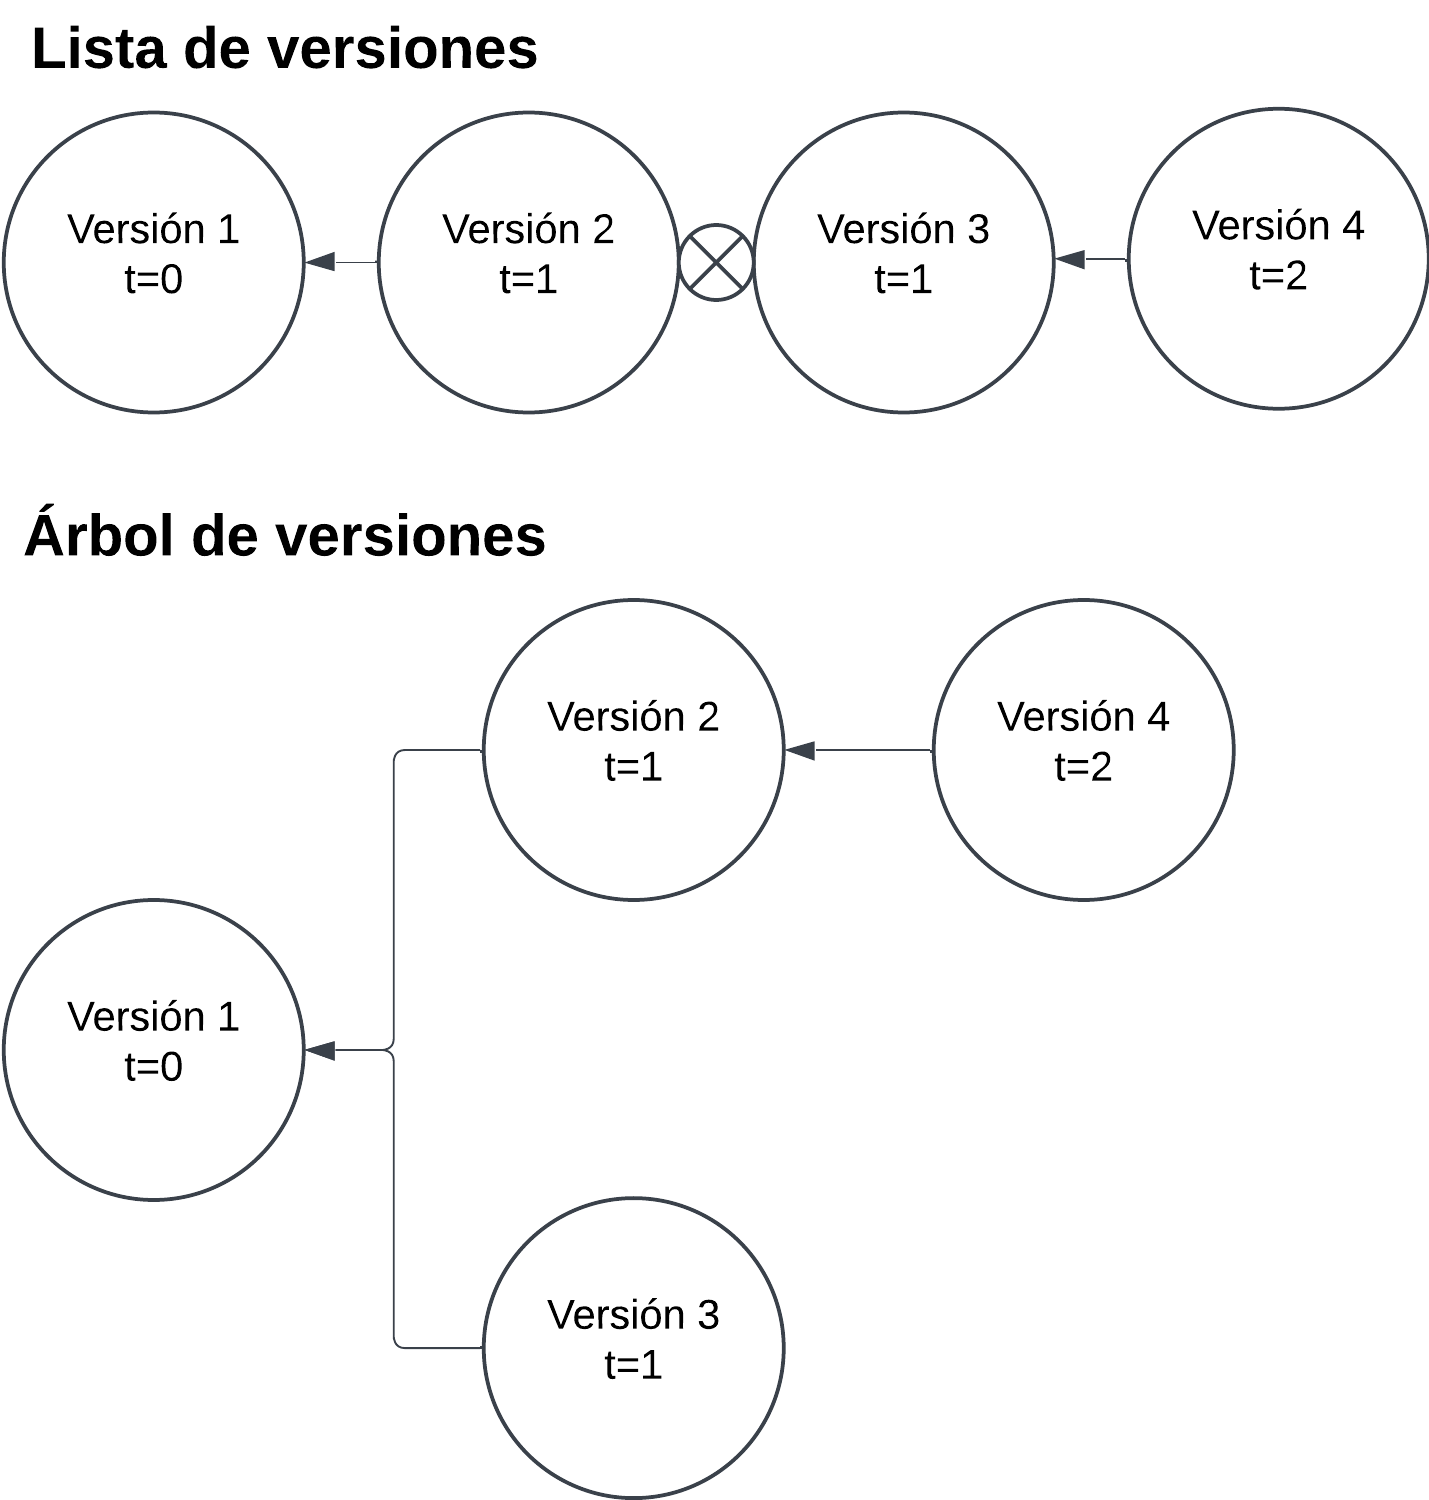
\includegraphics[width=0.5\linewidth]{img/solucion-wiki/arbol-versiones.png}
    \caption{Ambas maneras de almacenar versiones. En este caso, \texttt{t} es un momento en el tiempo en el que todas las bases de datos están sincronizadas. En el primer caso, cuando \texttt{t=1} en ambas versiones, significa que hay un conflicto ya que ambas se basan en la misma versión padre. En el árbol, ese problema se mitiga.}
    \label{fig:versions-tree}
\end{figure}

\paragraph{Elección de rama principal}

Una de las decisiones tomadas respecto al árbol de versiones, es que los usuarios sólo puedan modificar la última versión “principal”, es decir; un usuario no podrá editar en base a una versión arbitraria. Teniendo en cuenta esto, es fácil deducir que las ramas no principales o secundarias tendrán a lo sumo una versión en la mayoría de los casos. Esto es debido a que los demás usuarios que no hayan causado la colisión elegirán una rama principal, por lo tanto las demás ramas dejarán de recibir versiones nuevas. Elegir la rama de mayor cantidad de versiones será parte de la heurística para elegir la rama principal.

Sin embargo, esta decisión no es exhaustiva, ya que puede haber dos ramas con la misma longitud. De hecho, este caso es muy común debido a que dos usuarios que crean una nueva versión en base a la misma versión padre generan dos ramas del mismo tamaño. Para tomar una decisión que sea determinista e igual en todos los nodos, se decidió tomar la antigüedad de la última versión de cada rama como parámetro para la heurística. La rama mas antigua será considerada la rama principal. La antigüedad de una rama es decidida por una marca de tiempo o \textit{timestamp} grabada en el mismo nodo que crea la rama, y es enviado como parte de la versión a los demás nodos. Esto trae una desventaja en cuánto a seguridad, ya que un nodo puede falsificar un timestamp y así tener prioridad siempre, pero es mejorable utilizando algoritmos para crear timestamps en un sistema distribuido \cite{distributed-timestamps}.

\begin{figure}[H]
    \centering
    \begin{minipage}{0.9\linewidth}
        \lstset{
            basicstyle=\ttfamily\small,
            frame=single,
            captionpos=b
        }
        \begin{lstlisting}
type VersionID = string;

type Version = {
  id: VersionID;
  date: string;
  patch: Patch;
  parent: VersionID | null;
};\end{lstlisting}
    \end{minipage}
    \caption{Propiedades de una \texttt{Versión}}
    \label{fig:version-type}
\end{figure}

Una vez elegida la versión principal, se considera como rama principal a todas las versiones que entren en la cadena de padres, empezando por la versión principal hasta llegar a la versión raíz. De esta forma, sabemos que la rama principal siempre se podrá compilar, generando una red mucho más resiliente a cambios concurrentes. 
Por último, las versiones que no sean parte de la rama principal también podrán visualizarse. Se tomó esta decisión para permitir que los usuarios que hayan subido una versión por fuera de la rama principal puedan ver el contenido que editaron y, en todo caso, editar la nueva versión principal con el mismo.

\subsubsection{Arquitectura del mensajero en tiempo real}

La arquitectura para un mensajero es mucho más sencilla que la del repositorio de conocimiento. Consta de un grupo de chats, que a su vez contienen todos los mensajes. Cada mensaje contiene el texto enviado, el usuario que lo envió, un \textit{timestamp} del momento de su envío, entre otras cosas.

\paragraph{Aliases} En las implementaciones que se verán posteriormente, se determina que la manera de identificar a un usuario será mediante un ID similar a un hash en ambos casos. Esto es común para sistemas descentralizados, pero vuelve difícil diferenciar los usuarios en un chat. Para solucionar esto, se decidió agregar un alias que identifique al usuario, que no tenga que ser único y pueda ser cambiado. Su implementación varía dependiendo del ecosistema, pero en ambos es parte del objeto \texttt{ChatMessage} que almacena cada chat.

\paragraph{Respuestas} Se decidió identificar cada mensaje mediante un identificador, de manera tal que se pueda indicar el "padre" de un mensaje, o sea, el mensaje al que se le está respondiendo.

\begin{figure}[H]
    \centering
    \begin{minipage}{0.9\linewidth}
        \lstset{
            basicstyle=\ttfamily\small,
            frame=single,
            captionpos=b
        }
        \begin{lstlisting}
export type ChatMessage = {
  id: string;
  parentId: string;
  sender: string;
  senderAlias: string;
  message: string;
  timestamp: number;
};\end{lstlisting}
    \end{minipage}
    \caption{Propiedades de un \texttt{ChatMessage}}
    \label{fig:chat-message}
\end{figure}